%!TEX root = ../thesis.tex
% keep empty line

% keep empty line

% LEGE PAGINA OF TOEWIJDING OF LEUKE QUOTE OFZO

\newpage

\null

\pagebreak

% COLOPHON

% * Colophon and acknowledgement of funding
%     An inside page at the start of the thesis (colophon) describes where the work was done and who supported it. Funding bodies and granting agencies should be mentioned here. It is common to include logos of the University and associated research institutes. Several institutes have specific rules about the way the institute should be mentioned.
\newpage
% \null % only necessary if there is nothing before the vfill!

\begin{figure}[htbp!]
  \centering
  
\includegraphics[width=\textwidth]{ch_frontandback/img/RUG_FWN_KAPTEYN_logoEN_pms186.eps}
  % \caption{Caption here}
% \label{fig:figure1}
\end{figure}

\begin{figure}[htbp!]
  \centering
  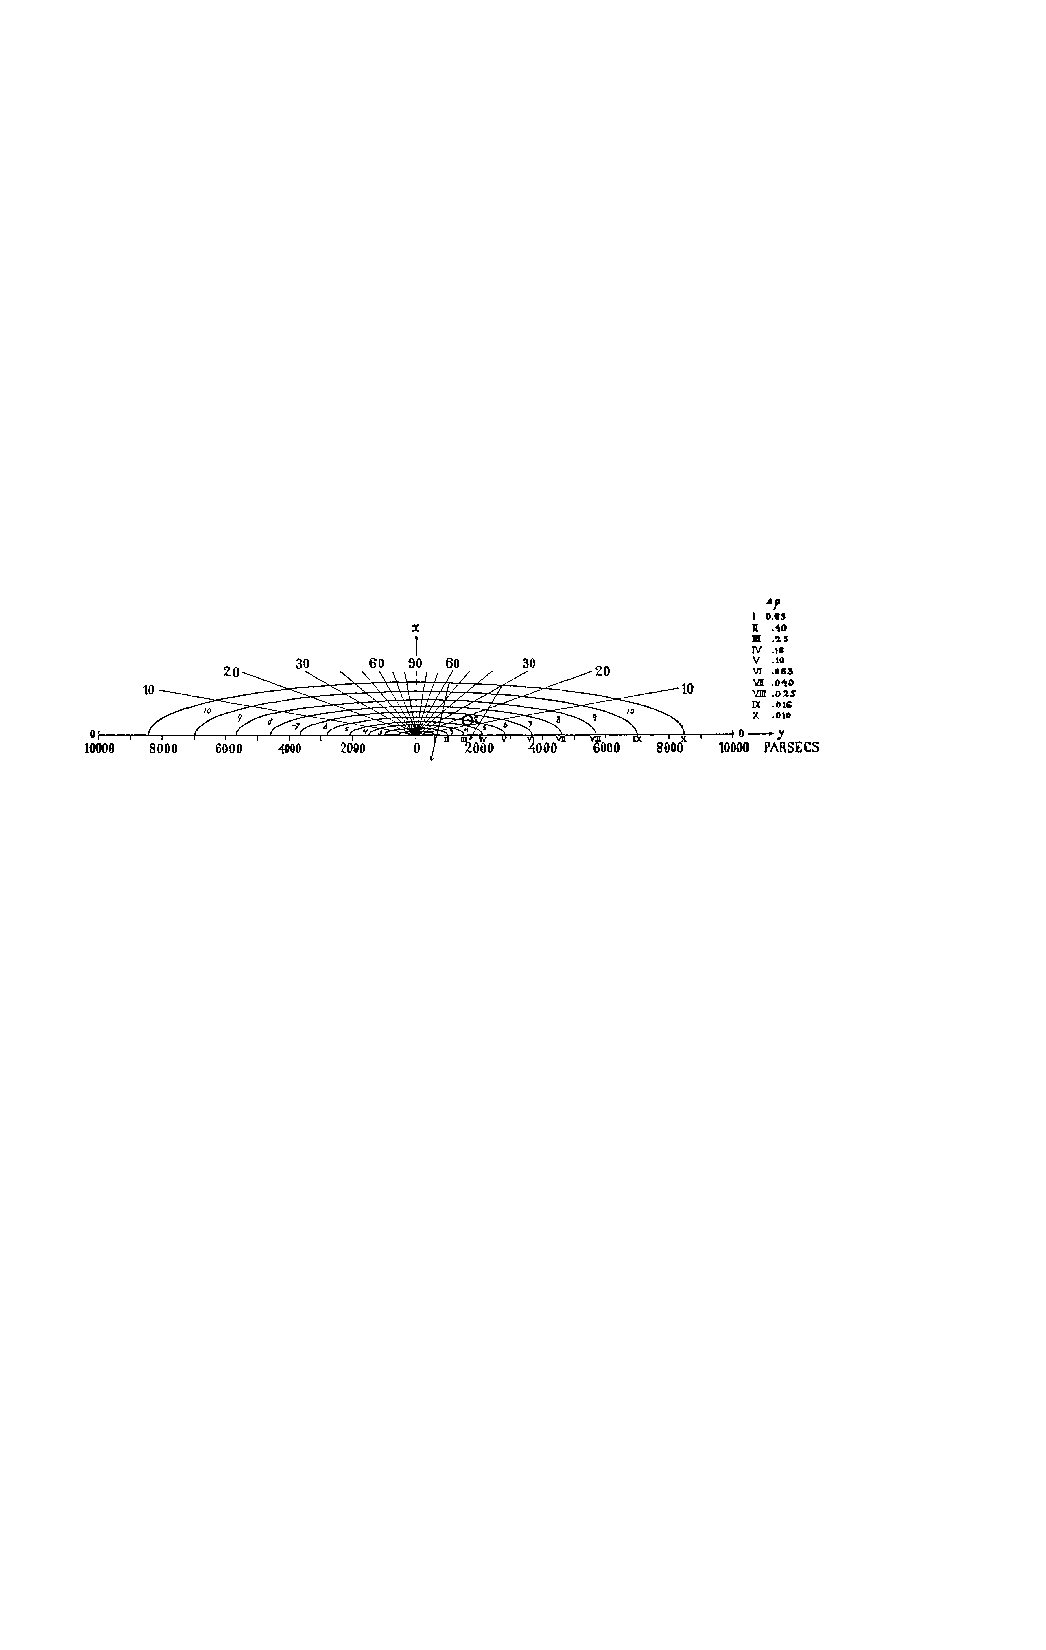
\includegraphics[width=\textwidth]{ch_frontandback/img/kapteynuniverse.pdf}
  % \caption{Caption here}
% \label{fig:figure1}
\end{figure}

\vfill

\textbf{Image above:}
The Kapteyn Universe \citep{1922ApJ....55..302K}, which consists of concentric ellipsoidal equidensity surfaces describing the distribution of stars.
The sun is indicated by the circle labeled ``S''.
I include this iconic image to highlight the contrast with our current, utterly uninspired logo, shown above.

\textbf{Front cover:}
The different parts of the cover image all show a differently filtered representation of the density field corresponding to the high-resolution $N$-body simulation of structure formation used in Chapter~\ref{ch:voidsde}.
The periodic field is repeated in both horizontal and vertical directions.
The full height of the cover spans about $857\mpc$ or about 2.8 billion light years or about 26,000,000,000,000,000,000,000 km.
The image shows the density in a slice with thickness $1.7\mpc$.
The density was computed using the \texttt{DTFE} method on a regular grid of $256 \times 256 \times 256$ cells, starting from $768^3$ dark matter particles.
The black-red-yellow bottom part shows the actual logarithmically scaled density values according to the `hot' color map of \texttt{Matplotlib} over the full range of density values.
At the top left, the \texttt{subfind} halo population with masses above $3\times10^{12} \msun$ is shown as circular profiles, representing clusters and groups of galaxies.
On the top right, we show the field's void population identified using the Watershed Void Finder.

\textbf{Back cover:}
The word cloud or, rather, word web was generated by randomly populating the part of the density field with values above $-0.8$ (the typical central void density) with all words from this thesis, filtered for stop words.
The size of the words depends on their frequency in this book.
Word web idea by Omar Choudhury.

Printed by Ipskamp Printing, Enschede.

This work was funded by NOVA project 10.1.3.07 and further supported by the Leids Kerkhoven-Bosscha Fonds and the Leibniz-Institut f\"{u}r Astrophysik Potsdam.

ISBN 978-90-367-9282-0 (printed version) \\
ISBN 978-90-367-9281-3 (electronic version)

\pagebreak

% optional: preface, see Harish's thesis for example
